\documentclass[../../main.tex]{subfiles}
\begin{document}
\onlyinsubfile{
\setcounter{chapter}{0}
}
\notinsubfile{}
\section{Werken op een quantumcomputer}\label{sec:wbQI}

\marginpar{\hfill\fbox{
\begin{minipage}[t]
{0.9\marginparwidth}naam:\hfill\vspace{1cm}
\end{minipage}
}}
\marginpar{\hfill\fbox{
\begin{minipage}[t]
{0.9\marginparwidth}klas:\hfill\vspace{1cm}
\end{minipage}
}}
\marginpar{\hfill\fbox{
\begin{minipage}[t]
{0.9\marginparwidth}datum:\hfill\vspace{1cm}
\end{minipage}
}}
We rekenen het voorbeeld~\ref{sec:XHZX} uit op de quantum computer Quantum Inspire in Delft. 
Wat is de uitkomst van \port{X}\port{H}\port{Z}\port{X}$\ket{0}$?

In deze opdracht ga je zelf een quantumcomputer programmeren. We maken gebruik van de quantumcomputer van Delft: Quantum-Inspire. Nu ja, als gast gebruik je gebruik je een simulatieprogramma. Wil je echt op de quantumcomputer dan kun je een account aanmaken. Voor deze opdracht is dat niet nodig. 
In figuur~\ref{fig:QIscreenshot} is een screenshot te zien van het programma voor je eerste opdracht.

\begin{flushleft}
\begin{minipage}{.35\textwidth}
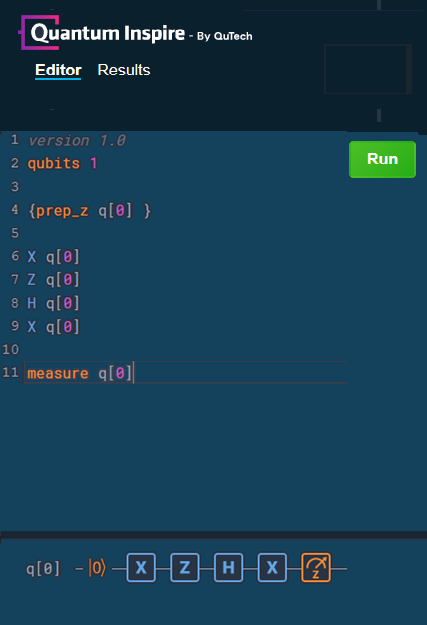
\includegraphics[width=\textwidth]{./img/QIscreenshot.png}
\end{minipage}%
\hfill
\begin{minipage}{.55\textwidth}
\captionof{figure}{De editor van de quantum-computer van Delft. Een programma kun je "runnen" (laten lopen). Daarna wordt je gevraagd om het aantal shots te kiezen. 
\label{fig:QIscreenshot}}
\end{minipage}
%\caption{E\'en vector in standaardbasis (rood) en diagonale basis.}\label{fig:hvad}
%\end{figure}
\end{flushleft}
\medskip
%\begin{opdracht}\label{opd:logica2}%
\begin{enumerate}
\item Ga naar de website van \href{https://www.quantum-inspire.com/}{Quantum Inspire}. Je krijgt een scherm met oranje-rode kleuren.
\item Klik rechtsboven de \texttt{Knowledge base} aan.
\item Links vind je de \texttt{quick guide} met het onderdeel \texttt{working with the editor} : klik aan.
\item Even scrollen en je ziet een voorbeeld met rechtsboven \texttt{open the editor}: klik aan. 
\href{https://www.quantum-inspire.com/projects/new?code=version\%201.0\%0Aqubits\%202\%0A\%0A\%7Bprep_z\%20q\%5B0\%5D\%20\%7C\%20prep_z\%20q\%5B1\%5D\%7D\%0A\%0A\%23\%20Create\%20a\%20superposition\%20state\%20for\%20qubit\%200\%0AH\%20q\%5B0\%5D\%0A\%0A\%23\%20Entangle\%20both\%20qubits\%20using\%20a\%20CNOT\%20gate\%0ACNOT\%20q\%5B0\%5D,\%20q\%5B1\%5D}{via deze  link}
\item Je bent nu in de editor met een programma dat al werkt.
\item Pas het programma aan zodat het overeenkomt met figuur~\ref{fig:QIscreenshot}.
\item Run het en zorg voor 1000 shots,
\item Bekijk de resultaten: voldoen ze aan je verwachting?
\item Herhaal de hele procedure voor een andere reeks poorten, bijvoorbeeld 
\port{X}\port{H}\port{X}\port{H}\port{X}$\ket{0}$
\end{enumerate}
%\end{opdracht}

\end{document}
